\documentclass[tikz]{standalone}
\usepackage{bm}
\usepackage{stix}

\usetikzlibrary{calc}

\definecolor{mplblue}{HTML}{1f77b4}
\definecolor{mplgreen}{HTML}{2ca02c}
\definecolor{mplmagenta}{HTML}{e377c2}

\tikzstyle{site}=[rounded corners, minimum size=0.8cm, inner sep=0, draw=mplblue!80!black, fill=mplblue!20!white]
\tikzstyle{sitex}=[rounded corners, minimum width=2cm, minimum height=0.8cm, inner sep=0, draw=mplgreen!80!black, fill=mplgreen!20!white]

\begin{document}
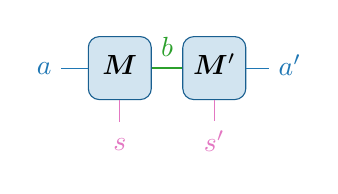
\begin{tikzpicture}[x=1.2cm, y=1.2cm]

\node [site] (x)  at (-0.5, 0) {\strut $\bm{M}$};
\node [site] (xp) at ( 0.5, 0) {\strut $\bm{M}'$};

\node [font=\vphantom{Ag}, text=mplblue   ] (a)  at (-1.3,  0  ) {$a$};
\node [font=\vphantom{Ag}, text=mplblue   ] (ap) at ( 1.3,  0  ) {$a'$};
\node [font=\vphantom{Ag}, text=mplgreen  ] (b)  at ( 0  ,  0.2) {$b$};
\node [font=\vphantom{Ag}, text=mplmagenta] (s)  at (-0.5, -0.8) {$s$};
\node [font=\vphantom{Ag}, text=mplmagenta] (sp) at ( 0.5, -0.8) {$s'$};

\draw [mplblue]         (x)  -- (a);
\draw [mplblue]         (xp) -- (ap);
\draw [mplgreen, thick] (x)  -- (xp);
\draw [mplmagenta]      (x)  -- (s);
\draw [mplmagenta]      (xp) -- (sp);

\end{tikzpicture}
\end{document}
